\documentclass[11pt]{scrartcl}
\usepackage[a4paper]{geometry}

\usepackage{graphicx}
%\graphicspath{ {./images/} }

\usepackage{fancyhdr}
\pagestyle{fancy}
\fancyhf{}
\fancyhead[L]{PULSOXYMETRIE} %Kopfzeile links
\fancyfoot[C]{\thepage}

\usepackage[utf8]{inputenc}
\usepackage{csquotes}
\usepackage[german]{babel}

\usepackage{setspace}

\usepackage{caption}
\usepackage{float}

\usepackage{hyperref}
\usepackage{pdfpages}

\hypersetup{
    pdftitle = {Pulsoxymetrie},
    pdfsubject = {Biomedizinischesystemtechnik Praktikum},
    pdfauthor = {Leona K{\"o}ck, Chris R{\"u}ttimann},
    pdfkeywords = {} ,
    pdfcreator = {pdflatex},
    pdfproducer = {LaTeX with hyperref}
}

\usepackage[
    style=apa,
    backend=biber,
    sortcites=false,
    sorting=none,
    hyperref=true,
    backref=false
]{biblatex}
\usepackage{amsmath}
\usepackage[T1]{fontenc}
\addbibresource{test.bib}

\setlength{\parindent}{0in}

\begin{document}
    \pagenumbering{Alph}
% ---------------------
% Titlepage
% ---------------------
    \begin{titlepage}
        \begin{center}
        {\LARGE OST Ostschweizer Fachhochschule}
            \\[1.5cm]
            \linespread{1.2}\large { Biomedizinischesystemtechnik Praktikum }

            \huge{\bfseries Pulsoxymetrie}
            \\%[1.5cm]
            \large{durchgef{\"u}hrt am 22. März 2021}
            \\[1.5cm]
   %         \linespread{1}
           
\includegraphics[width=8cm]{../images/ost_logo.eps}
           \\[1cm]
            {\small{Autoren}}\\
            {\Large{Leona K{\"o}ck}}\\
            {\Large{Chris R{\"u}ttimann}}
            \\[1cm]

            \vspace*{\fill}
            \large{\today}
        \end{center}

    \end{titlepage}

% ---------------------
% Abstract
% ---------------------
    \pagenumbering{Roman}
 %   \pdfbookmark[section]{Abstract}{abstract}
 %   \section*{Abstract}
    \addtocounter{section}{0}

 %   \pagebreak
    \setstretch{1.25}
% ---------------------
% Table of contents
% ---------------------
    \tableofcontents
    \pagebreak


% ---------------------
% Body
% ---------------------
    \pagenumbering{arabic}

    \section{Problem- und Zielvorstellung}
   Ziel dieses Praktikums war es, die Sauerstoffsättigung des Blutes mithilfe des Pulsoxymeter Frontend zu messen. 
   Dieselbe Messung sollte mit einem handelsüblichen Pulsoxymeter durchgeführt und verglichen werden.

    \section{Problemlösung}

    \subsection{Vorbereitung}
    Zur Vorbereitung wurden mithilfe des Dokuments \cite{Pulsoxymetrie} die folgenden Fragen beantwortet:
    
    \begin{itemize}
        \item[a]  Weshalb kann eine lebensgefährliche Kohlenmonoxid-Vergiftung über die
        Pulsoxymetrie nicht erkannt werden?
        \item[] Bei der Pulsoxymetrie wird ausgenutzt, dass beladene Hämaglobin, im Normalfall oxygeniertes Hämoglobin, %todo, hämaglobin vs hämoglobin?
        bei optischen Wellenlängen einen deutlich anderen Absorptionsverlauf als desoxygeniertes Hämoglobin.
        Es kann aber nicht unterschieden werden, welcher Stoff tatsächlich an das Hämoglobin gebunden ist.
        \item[b] Welche Bedingung müsste ein Pulsoxymeter erfüllen, um eine Kohlenmonoxid Vergiftung zu erkennen?
        \item[]  Die sogenannten CO-Oxymeter messen mit 4 bis 7 anstatt der sonst verwendeten 2 verschiedenen Wellenlängen und sind daher in der 
        Lage, Bindungen mit Kohlenmonoxid von Bindungen mit Sauerstoff optisch zu unterscheiden.
        \item[c] Wozu schaltet man im Messzyklus eine Dunkelphase ein? Was wird damit
        korrigiert?
        \item[] In der Dunkelphase werden die momentanen Störeinflüsse aus der Umgebung ermittelt und kompensiert.
        \item[d] Was ist die funktionelle und fraktionelle Sauerstoffsättigung?
        \item[] Funktionelle Sauerstoffsättigung: 
        \begin{equation}
            s_aO_2 = \frac{cO_2Hb}{cO_2Hb + cHb} 
        \end{equation}
        \item[] Fraktionelle Sauerstoffsättigung: hier werden alle Hb-Derivate gemessen, beispielsweise CO-Oxymeter
        \begin{equation}
            s_aO_2,func = \frac{cO_2Hb}{cO_2Hb + cHb + cCOHb + cMetHb + ...} 
        \end{equation}
        \item[e] In welcher Grössenordnung liegen die Messfehler der Pulsoxymeter und worin
        besteht dabei die Gefahr? 
        \item[] Die Hersteller geben die Genauigkeit beispielsweise mit 2\% im Sättigungsbereich über 90\% an.
        Da aber rund zwei Drittel der Messfälle zwischen 82 und 88\% fallen ist mit größeren Abweichungen zu rechnen. 
        Generell gilt zu beachten, dass es sich beim Pulsoxymeter um eine nichtinvasive Messmethode handelt,
        daher sollte nicht auf den Absolutwert, sondern auf die Messwertänderung geachtet werden.
    \end{itemize}

    Zusätzlich wurde das Blockschaltbild (\autoref{fig:block}) genauer untersucht.

    \begin{figure}[H]
        \centering
        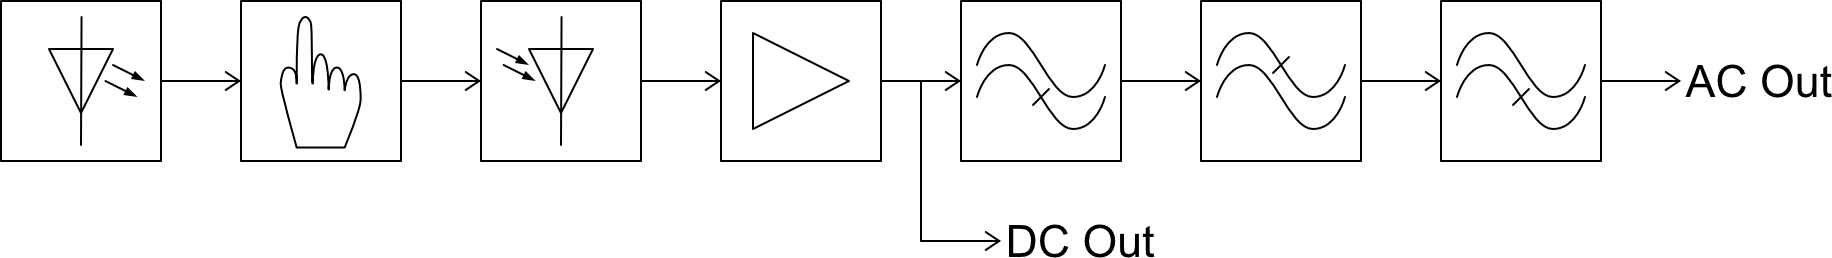
\includegraphics[width=15cm]{../images/Blockschaltbild}
        \caption{Blockschaltbild Pulsoxymeter Frontend, eigene Grafik}
        \label{fig:block}
    \end{figure}

    Das Polsoxymeter Frontend hat 2 LED's mit unterschiedlichen Wellenlängen.
    Diese werden über zwei Konstantstromquellen mit Strom versorgt.
    Sobald das Licht den Finger durchdrungen hat, wird es von einem Optischen Sensor in ein Signal umgewandelt.
    Im Blockschaltbild ist der Sensor durch eine Photodiode dargestellt, der Sensor selbst besteht aber aus weiteren Komponenten.
    Dieses Signal wird danach verstärkt und als DC Out ausgegeben.
    Dasselbe Signal läuft durch Hoch-, Tief- und wieder einen Hochpass, bevor es als AC Signal verwendet werden kann.
    Gemäss Schema gäbe es noch die Möglichkeit, dass Ausgangssignal des Optischen Sensors über einen Spannungsfolger direkt zu verwenden (RAW OUT), dies wurde jedoch in diesem Praktikum nicht benötigt.
    \\\\

    Für den Versuch wurden folgende Materialien benötigt:

    \begin{itemize}
        \item  Pulsoxymeter (kommerzielles Messgerät)
        \item Pulsoxymeter Frontend (Laboraufbau)
        \item Oszilloskop
        \item USB und BNC Kabel 
        
    \end{itemize}

    \subsection{Messung}
    Zuerst wurde jeweils mithilfe des Oszilloskops die Ausgangsspannung AC und DC am Pulsoxymeter Frontend bestimmt.
    Bewegungsartefakte galt es weitgehend zu vermeiden.\\
    Anschliessend wurde noch der Dunkelwert aufgenommen um die Einflüsse der Umgebung kompensieren zu können.
    Mithilfe der Formeln aus \cite{Pulsoxymetrie} konnte die Sauerstoffsättigung wie folgt ermittelt werden:
    \begin{equation}
        R = \frac{AC_{rot}}{DC_{rot} - Dunkelwert} 
    \end{equation}
    \begin{equation}
        IR = \frac{AC_{ifr}}{DC_{ifr} - Dunkelwert} \\
    \end{equation}
    \begin{equation}
        SaO_{2} = \frac{R}{IR} \\
    \end{equation}

    \section{Ergebnisse}
    Generell bereitete es Schwierigkeiten ein brauchbares Messergebnis zu erzeugen.
    Keine Bewegungsartefakte zu erzeugen war ein Ding der Unmöglichkeit, da einerseits für die Messung immer
    durchgehend ein Taster gedrückt werden musste, andererseits ist der Sensor für die Messung nur sehr klein und es
    gibt keine Ablagemöglichkeit, um den Finger für beide Messungen exakt gleich zu halten.\\
    Ein weiteres Hindernis waren Lichteinflüsse wie Deckenbeleuchtung oder die Sonne, die trotz aller
    Bemühungen nicht verhindert werden konnten.
    Teilweise konnten diese Einflüsse mit der Dunkelspannung kompensiert werden.

    \subsection{Proband Chris Rüttimann}
    \begin {table} [h]
    \centering
    \caption{Messergebnisse Pulsoxymetrie Frontend Chris}
    \label{tab:chris_frontend}
    \begin{tabular}{c|c c c}
        Messart & AC [mV] & DC [mV] & Puls [ms] \\
        \hline
        Infrarot & 926.5 & 195 & 955 \\
        Rot & 124 & 33 & 896 \\
        \hline
        Dunkelwert= 8mV \\
        R = 4.96\\
        IR = 4.95454\\
        $SaO_{2}$ = 100.1\%
    \end{tabular}  
    \end{table}

    \begin {table} [h]
    \centering
    \caption{Messergebnisse Pulsoxymeter Chris}
    \label{tab:chris_oxy}
    \begin{tabular}{c|c}
        $SpO_{2}$ & 97\%  \\
        BPM & 55 
    \end{tabular}  
    \end{table}
    Die Messung mit dem Pulsoxymeter war wie schon beschrieben sehr schwierig.
    Es benötigte viele Versuche um ein Ergebnis zu erhalten, das keine offensichtlichen Störgrössen enthielt.
    Die Berechnung der Sauerstoffsättigung ergab dann allerdings einen sehr unplausiblen Wert, da er über
    100\% liegt, siehe \autoref{tab:chris_frontend}.
    Diese Sättigung gibt eigentlich an, wie viel Prozent des gesamten Hämoglobins im Blut mit Sauerstoff beladen sind.
    Das können folglich nicht über 100\% sein.\\\\
    Die Messung mit dem handelsüblichen Pulsoxymeter erzielte ein schlüssiges Ergebnis mit einer
    Sauerstoffsättigung von 97\%, siehe \autoref{tab:chris_oxy}.\\
    Der Normwert für arterielles Blut liegt bei 94-97\%, bei jungen, gesunden Erwachsenen ein Wert nahe 100\%.

    \subsection{Proband Leona Köck}
    Wie auch beim ersten Proband war es hier wegen den Störeinflüssen nicht möglich, mit dem Frontend eine
    plausible Sauerstoffsättigung zu ermitteln.
    Der berechnet Wert von 210\% liegt nicht im gültigen Bereich.
    Mit dem handelsüblichen Pulsoxymeter konnte eine glaubwürdige Sättigung von 97\%, siehe
    \autoref{tab:leona_oxy}, ermittelt werden.

    \begin {table} [h]
    \centering
    \caption{Messergebnisse Pulsoxymetrie Frontend Leona}
    \label{tab:leona_frontend}
    \begin{tabular}{c|c c c}
        Messart & AC [mV] & DC [mV] & Puls [ms] \\
        \hline
        Infrarot & 241.8 & 360 & 765 \\
        Rot & 45.75 & 40 & 680 \\
        \hline
        Dunkelwert: 8.76mV \\
        R = 4.464  \\
        IR = 0.6884\\
        $SaO_{2}$ = 210\%
    \end{tabular}  
    \end{table}

    \begin {table} [h]
    \centering
    \caption{Messergebnisse Pulsoxymeter Leona}
    \label{tab:leona_oxy}
    \begin{tabular}{c|c}
        $SpO_2$ & 97 \%  \\
        \hline
        BPM & 87 
    \end{tabular}  
    \end{table}

    \section{Kritik und Anregungen}
	Es ist sehr spannend zu sehen, wie solch ein medizinischen Messgerät funktionieren und realtiv simpel nachgebaut
    werden können.\\
    Allerdings liefert das Pulsoxymeter Frontend keinerlei zuverlässige Messergebnisse und ist somit aus
    diagnostischer Sicht nicht ohne weitere Anpassungen zu brauchen.
    \pagebreak

    \section*{Eigenständigkeitserklärung}
    \addcontentsline{toc}{section}{Eigenständigkeitserklärung}

    Hiermit bestätigen wir, dass wir diesen Bericht selbstständig und ohne fremde Hilfe verfasst haben.
    Alle verwendeten Quellen wurden entsprechend dem APA-Standard gekennzeichnet.
    \\[3cm]


    \begin{figure}[H]
        
\includegraphics[width=4cm]{.././images/Unterschrift_Leona.png}
    \end{figure}
    \begin{tabular}{@{} l@{}}
        \hline \\
        \makebox[6cm]{Leona Köck}\\[2cm]
    \end{tabular}


    \begin{figure}[H]
        
\includegraphics[width=4cm]{.././images/Unterschrift_Chris.png}
    \end{figure}
    \begin{tabular}{@{} l@{}}
        \hline\\
        \makebox[6cm]{Chris Rüttimann}
    \end{tabular}

    \pagebreak
% ---------------------
% References
% ---------------------
    \printbibliography
    \addcontentsline{toc}{section}{Literaturverzeichnis}

% ---------------------
% List of figures
% ---------------------
%    \listoffigures
%    \addcontentsline{toc}{section}{Abbildungsverzeichnis}
%    \pagebreak

% ---------------------
% List of tables
% ---------------------
%\listoftables



% ---------------------
% Anhang
% ---------------------
%\appendix

\end{document}